%version of 01-21-20

\chapter{Solutions/Hints for selected exercises}
\label{ch:Exercises}



%\section*{Exercises: Chapter 2}

\begin{itemize}
\item
{\bf 2.2. Meeting people at a party}

{\em Some two attendees shake the same number of hands.}
\medskip

The pigeonhole principle guarantees that some two attendees shake the same
number of hands.  To wit, the number of people that each attendee {\em
  does not know} belongs to the set $\{ 0, 1, \ldots, 2n-2 \}$,
because each person knows him/herself and his/her partner.  

Since there are $2n$ handshakers (the pigeons) and $2n-1$ numbers of hands
to shake (the boxes), some two shakers must shake the same numbers of
hands. 
\medskip
\item
{\bf 2.4. Bi-colored necklaces in tubes}

A {\it necklace} is composed of $2n$ jewels: $2a$ black jewels and $2b$ white jewels. 
\ignore{************************
 For illustration, the necklace in Fig.~\ref{fig:sample-necklace} has $n = 6$, $a = 5$, and $b =1$.
\begin{figure}[ht]
\begin{center}
       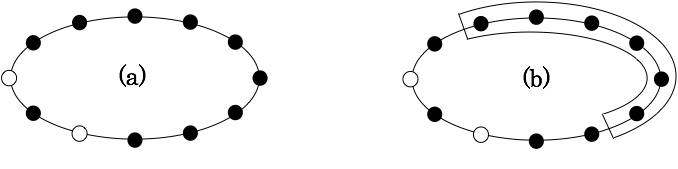
\includegraphics[scale=0.35]{FiguresMaths/SampleNecklace}
\caption{(a) A necklace having $12$ jewels: $10$ black and $2$ white.  (b) The necklace in a tube.}
\end{center}
\end{figure}

In part (a) of the figure, the necklace is unadorned; in part (b), the necklace appears within a length-$n$ {\it tube} which isolates one string---i.e., half-necklace---of $n$ jewels from the complementary string.
*******************************}
\smallskip

\noindent {\em For any bi-colored necklace, there is a way to position the tube so that inside the tube and outside the tube, 
there are equally many jewels, equally many black jewels, and equally many white jewels.} 
\smallskip

Slide the tube around the necklace, and count both black and white jewels at each step.  
How can these numbers change in a single step?
\smallskip

Let consider a position of the tube. 
The effect of a shift is to replace one jewel at the extremity of the tube by another jewel. 
If both jewels have the same color, the counting in unchanged while if they have different colors
(for instance, a black replaces a white), the number of whites decreases and the number of blacks increases. 
At the same time, the number of whites increases and the number of blacks decreases in the complementary 
remaining part of the necklace. 

\medskip \item
{\bf 2.6. Using {\em geometric} intuition to sum inverse powers of $4$}
\smallskip

We consider a variant of Proposition~\ref{thm:sumof-1/4-induction} where the focus is put on the entire infinite summation
\[ S \ \ = \ \  {1 \over 4} \ + \  {1 \over 4^2} \ + \cdots + \ {1 \over 4^k} \ + \cdots  \]

\smallskip

\ignore{***************
We prove in Proposition~\ref{thm:sum-finite-geometric-series}(b) that this infinite summation converges to the value ${1 \over 3}$.  
A simple way to see this is to multiply the summation $S$ term by term by the fraction $1/4$.  We observe---just by inspection---that the resulting product, which clearly has the value $S/4$, equals $S - 1/4$, so that $S = 1/3$.
\smallskip
*************************}

\begin{itemize}
\item
{\em prove that the four triangles are similar to one another.}
\smallskip

Let consider the small upper triangle and duplicate it twice.
Put both of them at the bottom of the original triangle
(as shown in Fig.~\ref{Fig:Sum1over4FirstLayer}(right)). 
There is another reversed triangle left at the middle of the figure (the white one). 
It has the same sides as the previous ones and its base is also half of the base of the original triangle,
thus it is also similar to the small upper triangle.

\begin{figure}
\begin{center}
        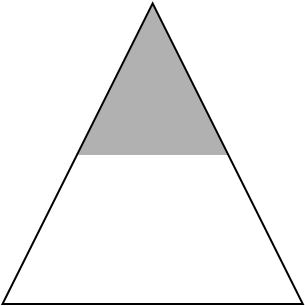
\includegraphics[scale=0.3]{FiguresMaths/Sum1over4topTriangle}
        \hspace{1cm}
        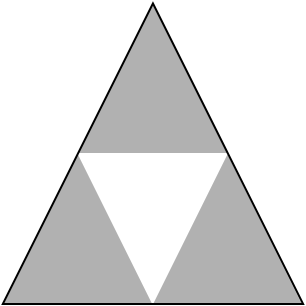
\includegraphics[scale=0.3]{FiguresMaths/Sum1over4similarTriangles}
        \caption{A sub-triangle at the top(left) and its two duplicates(right).
        These three traingles plus the white reserved one at the middle perfectly partition the area of the original big triangle.}
        \label{Fig:Sumgeosimilar}
\end{center}
\end{figure}

\item
{\em prove that the four triangles are similar to the original triangle.}
\smallskip

The small upper triangle has been obtained by divided by a factor of $2$ both the basis and the sides
of the original triangle (see Fig.~\ref{Fig:Sum1over4FirstLayer}(left)). 
Thus, it is similar to the original one. 
\smallskip

\item
{\em prove that the four triangles have area which is $1/4$ that of the original triangle.}

This comes directly from the two previous observations: The four triangles have the same area
and they exactly cover the original triangle. 
\end{itemize}

{\em Assemble these facts into an evaluation of the sum $S$.}
\smallskip

The sum $S$ is obtained by recursively applying the same process of partitioning again and again
on the small upper triangles. 
The whole process splits the original triangle into layers containing each $3$ sub-triangles
(see Fig.~\ref{Fig:Sum1over4FirstLayer}). 
As the three sub-triangles are the same, the area of the central reversed triangle is $\frac{1}{3}$ of the area of the layer. 
\begin{figure}
\begin{center}
        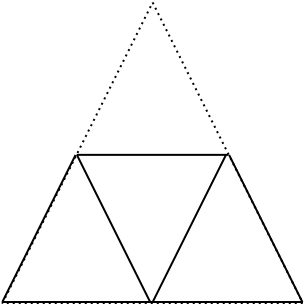
\includegraphics[scale=0.3]{FiguresMaths/Sum1over4FirstLayer}
        \caption{First bottom layer of the partitioning..}
        \label{Fig:Sum1over4FirstLayer}
\end{center}
\end{figure}

The final solution is depicted in Fig.~\ref{Fig:Sum1over4cascade} where the recursive process is applied \textit{ad libitum}. 

\begin{figure}
\begin{center}
        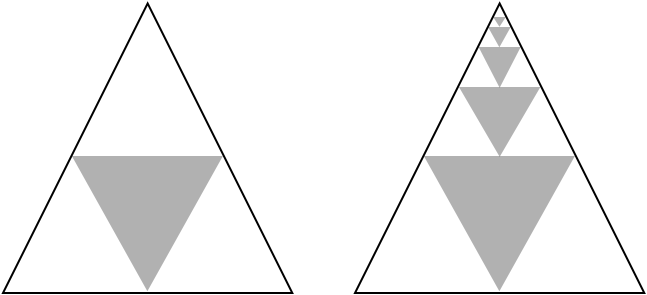
\includegraphics[scale=0.3]{FiguresMaths/Sum1over4cascade}
        \caption{Summary of the graphical construction. Assuming the total area is 1, the area of the grey internal triangle (left) is $\frac{1}{4}$.
        As the grey area is one third at each layer (right), the whole area is $\frac{1}{3}$.
        By the double counting Fubini's principle, this area is the sum of the $\frac{1}{4^k}$ (for $k \geq 1$).}
        \label{Fig:Sum1over4cascade}
\end{center}
\end{figure}

\end{itemize}

\ignore{*************************
\subsection{A graphical proof}

\noindent \textit{The problem.}
%\label{thm:an-arithmetic-identity}
Prove the following property:

or any positive integer $n$,
\[ \Delta_{2n-1} \ = \ n + 4 \Delta_{n-1}. \]
\medskip

\noindent \textit{The solution.}

Consider the arithmetic series in (\ref{eq:arith-seq}) for the case
$a=1$ and $b=4$.  
By Proposition~\ref{thm:sum-of-arithmetic-series},
this series, call it $S^{(1,4)}(n)$, has the sum
\begin{equation}
\label{eq:triangles}
S^{(1,4)}(n) \ = \ n + 4 \Delta_{n-1}.
\end{equation}

Let us represent the sum $\Delta_{n-1}$ in the natural way as a
triangle of tokens.  This triangle has a base of $n-1$ tokens, upon
which sits a row of $n-2$ tokens, upon which sits a row of $n-3$
tokens, \ldots, all the way to the apex, which has a single token.

Now, let us view equation (\ref{eq:triangles}) as giving us access to four
copies of the preceding triangle of tokens.  Let us arrange these
triangles in the manner depicted in Fig.~\ref{fig:Delta(n)4}.
\begin{figure}[ht]
\begin{center}
       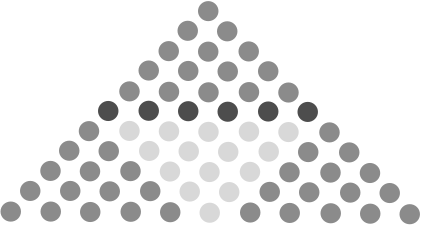
\includegraphics[scale=0.5]{FiguresMaths/Delta4}
 \caption{Arranging the four triangles plus a row to obtain a new (bigger) triangle.}
       \label{fig:Delta(n)4}
\end{center}
\end{figure}
Now, ``complete the picture'' by adding an ``extra'' row of $n$
tokens at row $n$ of the figure (these are depicted in dark gray in
the figure).  The four small triangles, augmented by the ``extra'' row
of $n$ tokens has clearly become a representation  of $\Delta_{2n-1}$
by tokens.

We now have a purely pictorial proof of the proposition. 

*************************}


%%%%%%%%%%%%%%%%%%%%%%%%%%%%%%%%%%%%%%%%%%%%%%


%\section*{Exercises of Chapter 3}

\begin{itemize}
\item
{\bf 3.8. More connections between strings and functions}
\medskip

{\em Craft an argument that predicts the number of permutations, based on the size of set $S$.}
\smallskip

\begin{itemize}
\item
As you create a new string of numbers, in how many ways can you choose {\em the first number}? 
{\em the second number}? \ldots
\item
Based on your answers for the first and second and third numbers of the new string, 
in how many ways can you choose {\em the first two numbers---i.e., the first {\em pair} of numbers}? 
{\em the next two numbers}? \ldots
\end{itemize}

{\em Strengthen your argument by listing all permutations of  $S' =  \{1,2,3,4,5\}$.}

\smallskip

Write small---there are a lot of permutations.

{\em Extrapolate from your argument to determine the number of permutations of the set 
$S" =  \{1,2,3, \ldots, n\}$, as a function of $n$.}

\end{itemize}


%%%%%%%%%%%%%%%%%%%%%%%%%%%%%%%%%%%%%%%%%%%%%%%%
%\section*{Exercises: Chapter 4}

\begin{itemize}
\item
{\bf 4.5. The rationals ($\Q$) and the integers ($\N$) are equinumerous}
\smallskip

{\em Provide a {\em detailed} proof of Proposition~\ref{thm:|Q|=|N|}.}  
Informally, there are equally many integers as there are rationals.
\end{itemize}


\ignore{***************************************
\subsection{Complex
  multiplication via $3$ real multiplications}
\index{complex number!multiplication via 3 real multiplications}

\noindent {\it The problem.}
%\label{thm:complex-mult-3real}
Show how to compute the product of two complex numbers using only {\em three}
real multiplications rather than four.
\medskip

\noindent {\it The solution.}
Although implementing (\ref{eq:complex-mult}) ``directly'' correctly
produces the product $\kappa = (a+bi) \cdot (c+di)$, there is another
implementation that is {\em more efficient}.  Specifically, the
following recipe computes $\kappa$ using only {\em three} real
multiplications instead of the four real multiplications of the
``direct'' implementation.  We begin to search for this recipe by
noting that our immediate goal is to compute both Re$(\kappa) = ac-bd$
and Im$(\kappa) = ad+bc$.  We can accomplish this by computing the
{\em three} real products
\begin{equation}
\label{eq:complex-mult-3a}
(a+b) \cdot (c+d); \ \ \ \ \
ac;  \ \ \ \ \ bd
\end{equation}
and then noting that
\begin{equation}
\label{eq:complex-mult-3b}
\begin{array}{lcl}
\mbox{Im}(\kappa) & = & (a+b) \cdot (c+d) - ac -bd, \\
\mbox{Re}(\kappa) & = & ac -bd
\end{array}
\end{equation}
We thereby achieve the result of the complex multiplication described
in (\ref{eq:complex-mult}) while using only {\em three} real
multiplications.


%%%
\subsection{Another proof for irrationality of $\sqrt{2}$}


\noindent \textit{The problem.}
Prove the irrationality of $\sqrt{2}$ using a geometrical argument.
\medskip

\noindent \textit{Hint.}
The proof is by contradiction. 

Consider $\sqrt{2}$ is rational, which means there exists a pair of integers $(a,b)$
such that $\sqrt{2} = \frac{a}{b}$ (where $a$ is larger than $b$).
Among all possible pairs, take the unique irreductible ratio.

Represent this expression geometrically by the corresponding isosceles triangle
which is the one of minimal surface. 

The contradiction comes by constructing another isosceles triangle with a smaller surface.
%Squaring this expression leads to $2.b^2 = a^2$.
\medskip

\noindent \textit{The solution.}

The solution is depicted in Fig.~\ref{Fig:sqrtbisInit} and~\ref{Fig:sqrtbisFin} . 
\begin{figure}
\begin{center}
        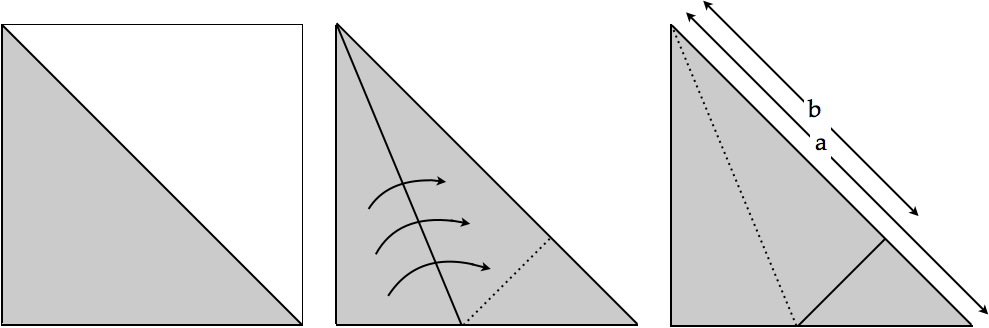
\includegraphics[scale=0.3]{FiguresArithmetic/sqrtbisInit}
        \caption{First step: folding the triangle along the side.}
        \label{Fig:sqrtbisInit}
\end{center}
\end{figure}
\begin{figure}
\begin{center}
        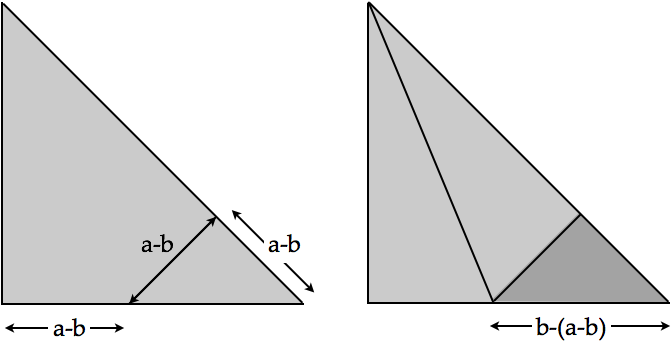
\includegraphics[scale=0.3]{FiguresArithmetic/sqrtbisFin}
        \caption{Second step. The sides of the small isosceles triangle are integers.}
        \label{Fig:sqrtbisFin}
\end{center}
\end{figure}
****************************}


%%%%%%%%%%%%%%%%%%%%%%%%%%%%%%%%

\ignore{*******************************
\section{Chapter 5}


\subsection{A ``trick'' for squaring certain integers}


\noindent \textit{The problem:}

Let $n$ be any number that has a $2$-digit decimal numeral of the form

\hspace{.25in}$5.\delta$ \ \ \ \ $(\delta \in \{ 0,1,2,3,4,5,6,7,8,9\})$.

\noindent
Then the square of $n$ is the integer

\hspace{.25in}$25 \ + \ \delta \cdot (\delta +1)$
\medskip

\noindent \textit{The solution:}

We can rewrite the premise of the proposition in the form
\[ n \ = \ 10 \cdot \delta + 5 \]
It is now easy to invoke Proposition~\ref{prop:(a+b)(c+d)} and the
distributive law to compute that

\[ n^2 \ = \ 100 \cdot \delta \cdot (\delta+1) + 25 \]
To wit: 
\[
\begin{array}{lclll}
n^2 & = & (10 \cdot \delta + 5)^2 & & \mbox{Given} \\
    & = & 100 \cdot \delta^2 \ + \ 100 \cdot \delta \ + \ 25
              & & \mbox{the proposition} \\
    & = & 100 \cdot (\delta^2 \ + \ \delta) \ + \ 25
              & & \mbox{factoring: distributive law} \\
    & = & 100 \cdot \delta \cdot (\delta + 1) \ + \ 25
              & & \mbox{factoring: distributive law} \\
\end{array}
\]
A parlor trick has become a mathematical demonstration!


%%%
\subsection{Revisiting a very old problem}

\noindent \textit{The problem:}

This problem comes from babylonians in the 18th century BC.
The numeral system was in base 60, and the problem was to determine the length of the side of a square which was part of a larger rectangle.
The following figure details the process.
\medskip

\noindent \textit{The solution:}

The idea of the proof is to represent the left hand side by the square $x^2$ beside a rectangle $60 \times x$
(see Fig.~\ref{fig:equationBabillon}).
Recall that the coefficient of $x$ in the equation is $1$, this corresponds to $60$ in the considered basis. 
Then, split the right rectangle into two equal parts and move one part a the bottom of the left square.
The final figure shows the whole square whose surface is equal to $45$ plus the surface of the white square
whose surface is equal to $30 \times 30$.
In base $60$, this is equal to $15$. 
$45+15 = 60$, thus, the big square is the unit square, its side is $60$.
Thus, the length of the initial square is equal to $60-30=30$.
\begin{figure}[htb]
\begin{center}
       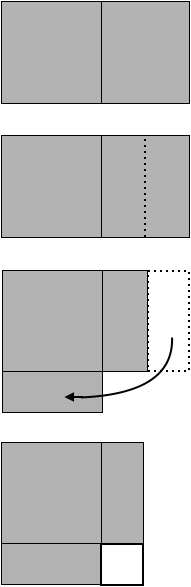
\includegraphics[scale=0.4]{FiguresArithmetic/tabletteMesopotamie}
\caption{Solving $x^2 + x = 45$.}
\label{fig:equationBabillon}
\end{center}
\end{figure}
*****************************}


%%%%%%%%%%%%%%%%%%%%%%%%%%%%%%%%%%%%%%%%%%

%\section*{Exercises: Chapter 6}

\begin{itemize}
\item
{\bf 6.4. Evaluating $S_1(n) = \sum_{i=1}^n \ i$, using the fact that $S_2(n) = \sum_{i=1}^n \ i^2$}
\smallskip

{\em Show how to use this machine in order to compute the sum of the first $n$ integers.}

\medskip
The idea here is to write the sum by extracting the two extreme terms of the sum of squares at rank $n+1$ (namely, first and the last element).

\begin{eqnarray*}
S_2(n+1) & = &  \sum_{i=1}^{n} i^2 \ + \ (n+1)^2  \\
 & = & S_2(n) \ + \ (n+1)^2 \\
S_2(n+1) & = &  1 \ + \sum_{i=2}^{n+1} i^2 \\
 & = &  1 \ + \sum_{i=1}^{n} \ (i+1)^2 \\
 & = &  1 \ + \sum_{i=1}^{n} \ (i^2 \ + \ 2.i \ + \ 1) \\
 & = & 1 \ + \ S_2(n) \ + \ 2.S_1(n) \ + n
\end{eqnarray*} 
The term $S_2(n)$ disappears while considering both expressions of $S_2(n+1)$:
\begin{eqnarray*}
 S_2(n) \ + \ (n+1)^2 & = & 1 \ + \ S_2(n) \ + \ 2.S_1(n) \ + n \\
 (n+1)^2 & = & 1 \ + \ 2.S_1(n) \ + n \\
 2.S_1(n) & = & (n+1)^2 \ - \ (n + 1) \\
 S_1(n) & =  & \frac{1}{2} \ n(n+1) 
\end{eqnarray*} 
\medskip

\item
{\bf 6.6. Evaluating a geometric summation pictorially}
\smallskip

\ignore{***************
In Section~\ref{sec:summing-geometric-series:techniques}, we used Thales's theorem about similarity in triangles (Theorem~\ref{thm:Thm-of-Thales-similarity}) to sum the simple infinite geometric series $\sum_{i=0}^\infty \ b^i$.  It turns out that a modest modification of that evaluation strategy allows us also to evaluate the truncated versions of that series, namely, the summations
\[ S^{(b)}(n) \ = \ \sum_{i=0}^n \ b^i \]
************************}

{\em Use the following figure to evaluate the following expression.}
\[ S^{(b)}(n) \ = \ \sum_{i=0}^n \ b^i \]

\centerline{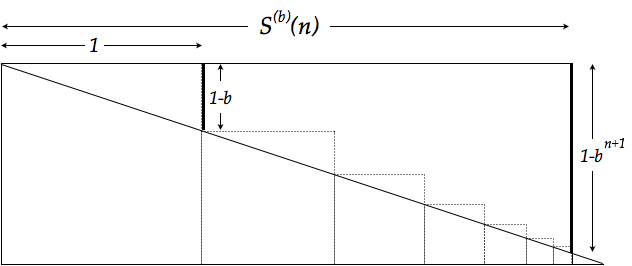
\includegraphics[scale=0.4]{FiguresArithmetic/ThalesGeometricSumFiniteSol}}
\smallskip

We use Thales's theorem (\ref{thm:Thm-of-Thales-similarity}) in the two upper similar triangles .
\[ \frac{S^{(b)}(n)}{1-b^{n+1}} \ = \ \frac{1}{1-b} \]
\[ S^{(b)}(n) \ = \ \frac{1-b^{n+1}}{1-b} \]

\medskip

\item
{\bf 6.7. A direct proof that the harmonic series diverges}

{\em Develop a proof of the divergence of the harmonic series 
\[ S^{(H)} \ = \ \sum_{k=1}^\infty \ {1 \over k} \]
\begin{itemize}
\item
partitioning $S^{(H)}$'s terms into groups whose sizes are successive powers of $2$
\item
developing an argument based on the sums within the groups.
\end{itemize}
}

\smallskip

The partitioning step operates as follows:
{\footnotesize
\[ 
\begin{array}{ll}
S^{(H)}   & = \ 1  + {1 \over 2} + \left(  {1 \over 3}   +  {1 \over 4}  \right) + \left( {1 \over 5} + {1 \over 6}+ {1 \over 7}  +  {1 \over 8} \right) + \left( {1 \over 9} + {1 \over 10}+ {1 \over 11}  +{1 \over 12} + {1 \over 13} + {1 \over 14} + {1 \over 15} + {1 \over 16} \right) \ +\cdots
\end{array} \]
}

More precisely, each group, say $G_i$, is composed by the $i$ integers from $\frac{1}{2^{(i-1)}+1}$ to $\frac{1}{2^{i}}$ 
(for $i \geq 1$).
Grouping the terms like before, the sum within each group $G_i$ is greater than $\frac{1}{2}$:
\[ 
\begin{array}{l}
{1 \over 3} + {1 \over 4}  > 2.{1 \over 4} = {1 \over 2} \\ \smallskip
{1 \over 5} + {1 \over 6} + {1 \over 7}+ {1 \over 8}  > 4.{1 \over 8} = {1 \over 2}  \\  \smallskip
{1 \over 9} + {1 \over 10} + {1 \over 11}  +{1 \over 12} + {1 \over 13} + {1 \over 14} + {1 \over 15} + {1 \over 16}  > 8.{1 \over 16} = {1 \over 2}  \\  \smallskip
\cdots
\end{array} \]
Thus, 
\[ 
\begin{array}{ll}
S^{(H)} \ > \ 1 \ + \ \left( {1 \over 2} \ + \ {1 \over 2} \right) \ + \left( {1 \over 2} + {1 \over 2} \right) + \cdots
\end{array} \]
$S^{(H)}$ is greater than the infinite sum of 1 and thus, it is unbounded .

\medskip

{\em Propose an alternative analysis by changing the groupings where the terms are gathered 3 by 3}
\[ 
\begin{array}{ll}
S_i & = \left( \frac{1}{3i-1} + \frac{1}{3i} + \frac{1}{3i+1} \right) 
\end{array} \]
\[ 
\begin{array}{ll}
S^{(H)}  & = 1 + S_1 +  \cdots + S_i + \cdots  > 1 + 3.\frac{1}{3} + 3.\frac{1}{6} + \cdots + 3.\frac{1}{3i} + \cdots
\end{array} \]

since $S_i > 3.\frac{1}{i} $

The proof is by contradiction:
if $S^{(H)} $ is finite, from the previous relation we have: $S^{(H)}  > 1 + S^{(H)} $, which is obviously impossible.
\medskip

\item
{\bf 6.8. Summations, and summations of summations}
\smallskip

  \begin{itemize}
  \item a.
{\em Prove that}
\[ \widehat{\Theta}_n \ \eqdef \  \sum_{k=1}^n \ \Delta_k \ = \   
\Delta_1 + \Delta_2 + \cdots + \Delta_n \ = \ \frac{1}{3} \Delta_n \cdot (n+2) \]

The result is obtained by replacing the $\Delta_k$ by their expression within the sum
and using the developed expression of the sum of squares:
\begin{eqnarray*}
\widehat{\Theta}_n & = & \sum_{k=1}^n \ \frac{k.(k+1)}{2} \\
 & = & \frac{1}{2} \sum_{k=1}^n k^2  + \frac{1}{2} \sum_{k=1}^n k  \\
 & = & \frac{1}{2} \ \left( \frac{n.(2n+1).(n+1)}{6} \ + \ \frac{n.(n+1)}{2} \right)\\
 & = & \frac{1}{2} \frac{n.(n+1)}{2} \left( \frac{2n+1}{3} + 1 \right)  \\
 & = & \frac{1}{2} \Delta_n \frac{(2n+4)}{3}  \\
  & = & \Delta_n \frac{(n+2)}{3}  \\
\end{eqnarray*} 

%  \item
%{\em Develop and verify a formula for the summation:}
%\[ \Upsilon_n  \ \eqdef \  \sum_{k=1}^n \ \widehat{T}_k \ = \  
%\widehat{T}_1 + \widehat{T}_2 + \cdots + \widehat{T}_n \]

  \item b.
{\em Prove the following identities involving $\Delta_n$.  For all $n \in \N^+$:}
    \begin{itemize}
    \item i.
$\Delta_n \ + \ \Delta_{n-1} \ = \ n^2$

\smallskip
The pictorial proof is obtained by a slightly modified scheme as for the expression of $\Delta_n$. 
\begin{figure}[htb]
\begin{center}
       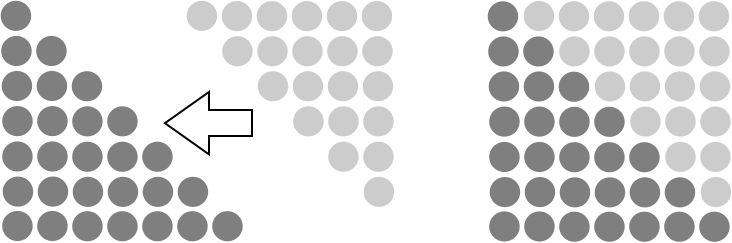
\includegraphics[scale=0.35]{FiguresMaths/DeltaSumSquare}
\caption{process of summing two consecutive $\Delta_n$(left) and the concatenation as a $n$ by $n$ square(right).}
%\label{fig:}
\end{center}
\end{figure}


 \item ii.
$\Delta_n^2 \ - \ \Delta_{n-1}^2 \ = \ n^3$

\smallskip

Write $\Delta_n \ = \ n \ + \ \Delta_{n-1}$ and replace it in the expression.
\begin{eqnarray*}
\Delta_n^2 \ - \ \Delta_{n-1}^2 & = & \left( n \ + \ \Delta_{n-1} \right)^2 - \ \Delta_{n-1}^2  \\
 & = & n^2 \ + \ 2n.\Delta_{n-1} \ + \ \Delta_{n-1}^2 - \ \Delta_{n-1}^2 \\
 & = & n^2 \ + \ 2.n\frac{n(n-1)}{2}\\
 & = & n^2 + n^3 - n^2 \\
\end{eqnarray*} 

\end{itemize}

  \item c.
{\em Derive a closed-form expression for the sum}
\[ \widehat{\Theta}_n \ + \ \widehat{\Theta} _{n-1} \]

This question is more open here than the previous ones since we don't know \textit{what} to look for.
\smallskip

A way to study this problem is to come back to the original definition of the $\Theta_n$
as the sum of $\Delta_k$.
\begin{eqnarray*}
\widehat{\Theta}_n \ + \ \widehat{\Theta} _{n-1}  & = & \sum_{k=1}^n \Delta_k + \sum_{k=1}^{n-1} \Delta_k \\
 & = & \Delta_1 + \sum_{k=2}^{n} \left( \Delta_k + \Delta_{k-1} \right)
\end{eqnarray*} 
We use the previous expression of the sum of two consecutive $\Delta_k$
\[
\widehat{\Theta}_n \ + \ \widehat{\Theta} _{n-1} = 1 + \sum_{k=2}^{n} k^2  = \sum_{k=1}^{n} k^2 
\]
We can finally replace this sum by its closed-form expression.
\[
\sum_{k=1}^{n} k^2 = \frac{n(n+1)(2n+1)}{6}
\]

\end{itemize}
\end{itemize} 


\ignore{*****************************
%%%
\subsection{Sum of perfect cubes}

\noindent \textit{The problem.}
Show that the sum of $n$ first cubes is equal to a perfect square, and more precisely, $\Delta_n^2$.
\medskip

\noindent \textit{The solution.}
The proof is based on an hold and simple pattern that we learned in elementary school.
\medskip

\index{$n^2$ as sum of first $n$ odd integers!a proof from elementary school}

%
Consider the following reasoning which emerges from the way
multiplication tables are developed in elementary school.  
Let us first illustrate the idea using the case $n=5$.
\begin{equation}
\label{eq:Fubini-table}
\begin{array}{rrrrr}
1  &  2 &  3 &  4 &  5 \\
2  &  4 &  6 &  8 & 10 \\
3  &  6 &  9 & 12 & 15 \\
4  &  8 & 12 & 16 & 20 \\
5  & 10 & 15 & 20 & 25 \\
\end{array}
\end{equation}
Write the integers $1, 2, \ldots, n$ in a row.  Below this row, write
the doubles of these integers.  Below the ``double'' row, write the
triples of the integers.  Below the ``triple'' row, write the
quadruples of the integers, then the quintuples, and so on.  Note that
the resulting table is {\em symmetric:} its rows are identical to its
columns.
\medskip

Using again Fubini's rearrangement stratagem, we now count all the integers in
the table in two different ways.
\begin{enumerate}
\item
We sum the entries of our table by peeling away successively larger
reversed instances of the letter ``$L$'' (as in our earlier
``pictorial'' proof of
Proposition~\ref{thm:squares-odd-integers-Gauss}).  We find that the
integers in each ``$L$'' sum to a perfect cube.
Actually, the diagonal is (by definition) equals to the square.
\[
\begin{array}{rrrrrrrrr|rrc}
1  &    &    &    &    &   &     &    &   & 1   & = 1^3 \\
2  &  4 &  2 &    &    &   &     &    &   & 8   & = 2^3 \\
3  &  6 &  9 &  6 &  3 &   &     &    &   & 27  & = 3^3 \\
4  &  8 & 12 & 16 & 12 &  8 &  4 &    &   & 64  & = 4^3 \\
5  & 10 & 15 & 20 & 25 & 20 & 15 & 10 & 5 & 125 & = 5^3
\end{array}
\]

\item
We sum the successive rows of the $n \times n$ table (\ref{eq:Fubini-table}).  
The first row of the table sums to $\Delta_n$; the second row sums to $2
\Delta_n$; the third row sums to $3 \Delta_n$; \ldots; the last row sums
to $n \Delta_n$.  
Thus, the aggregate sum of the table's rows is 
\[ (1 + 2 + \cdots + n) \cdot \Delta_n \ = \ \left(\Delta_n \right)^2 \]
\end{enumerate}
We conclude that
\[
\sum_{i=1}^n i^3 \ = \  \left(\Delta_n \right)^2
\]
************************************************}


%%%%%%%%%%%%%%%%%%%%%%%%%%%%%%%%%%%%%

%\section*{Exercises: Chapter 7}


\ignore{****************************
\subsection{Handling asymptotic}


\noindent \textit{The problem.}

Prove that $f = O(g)$ and $h = O(k)$ for functions $f,g,h,k$ implies that
$f+h = O(g+k)$


\subsection{What's wrong?}

\noindent \textit{The aim.}
to investigate a proof which leads to surprising results.


\begin{enumerate}
\item
Let consider the infinite sum $A = 1-1+1-1+ \ldots$

show that $A=\frac{1}{2}$ (hint: compute $1-A$)
\item
Let now consider the other infinite sum $B=2-3+4-5+6 \ldots$

show that $B=\frac{1}{4}$ (hint: compute $A+B-1$)
\item 
Compute the sum of the integers $C=1+2+3+4+ \ldots$

show that $C=-\frac{1}{12}$ (hint: compute $C-B=4+8+12+16+ \ldots$)
\end{enumerate}

\medskip

\noindent \textit{The problem.}

What's wrong?

\medskip

\noindent \textit{The solution.}
First, summing up positive number should be positive, 
and second, the sum of the integers should be infinite...

Then, how to analyze the previous result/proof?
******************************************************}




%%%%%%%%%%%%%%%%%%%%%%%%%%%%%%%%%%


%\section*{Exercises: Chapter 8}

\begin{itemize}

\item
{\bf 8.2. Discovering fractal-like structure in Pascal's triangle}

\ignore{************************
Modular arithmetic can do wondrous, unexpected things with regular structures.  If one takes a system whose structure is governed by arithmetic and substitutes {\em modular} arithmetic for ordinary arithmetic, then the system's structure is somehow going to be ``folded into itself".  We illustrate this fact within a rather complex framework in Appendix~\ref{Appendix:tree-DB}; the ``folded" structures there are trees.  We illustrate the fact within a rather elementary framework in this exercise; the ``folded" structures here arise from Pascal's triangle.

\medskip
*************************}

The Pascal's triangle modulo a prime $m$ (where each of the triangle's entries are taken modulo $m$) is illustrated in Fig.~\ref{fig:TriangleFractal},
%Figs.~\ref{fig:TriangleModulo5raw} and~\ref{fig:TriangleModulo5shade}.
\begin{figure}[ht]
\begin{center}
	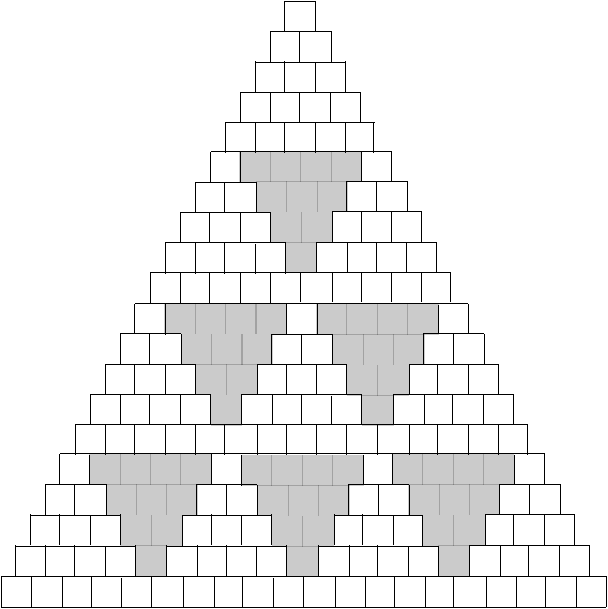
\includegraphics[scale=0.3]{FiguresArithmetic/PascalTriangleFractal.png}
	        \caption{The reproducible patterns in Pascal's triangle modulo $5$.
	        the shaded reversed triangles correspond to the input $0$.}
        \label{fig:TriangleFractal}
\end{center}
\end{figure}

The first $m$ levels of the triangle are replicated endlessly, with periodic inverted $(m-1)$-level triangles whose entries are all $0$.  (In the figure, the inverted triangle of $0$s is depicted in grey.) 
The original triangle has been transformed into a fractal-like repetitive structure whose pattern of repetitions is dictated by the parameter $m$.

\medskip

{\em Prove that the described transformation occurs.}

%
\medskip\item
{\bf 8.4. Divisibility among integers: via the Fundamental Theorem of Arithmetic}

  \begin{itemize}
\item
b. {\bf The sieve of Eratosthenes and its implications}

We formulate the sieve as a regimen for labeling integers with their prime factors.  For simplicity, we use the label $\lambda_p$ to identify integers which are multiples of prime $p$.
\medskip

The multiples of $2$, $3$ and $5$ are labeled in the following table:

$\begin{array}{c|c|c|c|c|c|c|c|c|c|c|c|c}
1 & 2 & 3 & 4 & 5 & 6 & 7 & 8 & 9 & 10 & 11 & 12 & 13 \\
 & \lambda_2 & & \lambda_2 & & \lambda_2 & & \lambda_2 & & \lambda_2 & & \lambda_2 & \\
 & & \lambda_3 & &  & \lambda_3 & & & \lambda_3 & & & \lambda_3 & \\
 & & & & \lambda_5 & & & & & \lambda_5 & & & 
\end{array}$ \ldots

\bigskip

{\em Prove the following results.}
     \begin{enumerate}
     \item
{\em 
Every integer $n>1$ is divisible by at least one prime number.
}

     \medskip\item
{\em 
Every sequence $k+1, \ldots, k+p$ of $p$ integers contains a multiple of $p$.
}

      \medskip\item This result calls for ``second-order" insights from the sieve.
{\em 
Every product of four consecutive integers, $(k+1) \cdot (k+2) \cdot (k+3) \cdot (k+4)$ is divisible by $4!$
}
\smallskip

We prove this result by a simple case by case analysis:
Any four consecutive integers contain exactly two consecutive even numbers.
Two such numbers are multiples of $2 \times 4 = 8$.
Moreover, three consecutive contains also a multiple of $3$. 
\smallskip

{\em Extend this exercise to divisors other than $4$.}
\smallskip

We prove by a similar analysis that the product of any $p$ consecutive integers is a multiple of $p!$.

\medskip\item
The sieve affords us an alternative proof that there are infinitely many primes, particularly via the alternative version that is due to Leonhard Euler.  In this version of the sieve, each prime and all of its multiples are removed from the sieve as soon as their existence is acknowledged.  Our earlier construction of Eratosthenes's version of the sieve now becomes:

\medskip

$\begin{array}{|l||c|c|c|c|c|c|c|c|c|c|c|c|c|c|}
\hline
\mbox{Initial array:} &
1 & 2 & 3 & 4 & 5 & 6 & 7 & 8 & 9 & 10 & 11 & 12 & 13 & \cdots \\
\mbox{after prime $2$ is processed:} &
1 &  & 3 &  & 5 &  & 7 &  & 9 &  & 11 &  & 13 & \cdots \\
\mbox{after primes $2, 3$ are processed:} &
1 &  &  &  & 5 &  & 7 &  &  &  & 11 &  & 13 & \cdots \\
\mbox{after primes $2, 3, 5$ are processed:} &
1 &  &  &  &  &  & 7 &  &  &  & 11 &  & 13 & \cdots \\
\hspace*{.8in} \vdots  &
 &  &  &  &  &  & \vdots &  &  &  &  &  &  & \\
\hline
\end{array}$

\bigskip

{\em Use Euler's sieve to prove that there are infinitely many primes.}
\medskip

{\em Hint:} If there were only finitely many primes, then at some (finite) stage in processing the sieve, the list of integers would be reduced to the single integer $1$.
\end{enumerate}
\end{itemize}

 \medskip\item

{\bf 8.5. The ``density"  of divisible pairs of numbers}

{\em Prove that the following assertion is true for every positive integer $n$.}
\medskip

{\em 
For every positive integer $n$:  If you remove {\em any} $n+1$ integers from the set $S = \{ 1, 2, \ldots, 2n\}$, then the set of removed integers contains at least one pair $p$ and $q > p$ such that $p$ divides $q$.
}
\medskip

Let $\alpha_i$ be the elements of this set of $n+1$ elements.

The $2n$ numbers of the sequence are decomposed into groups according to multiples of powers of $2$.
When there are multiple ways to write a number (for instance $12$ is equal to $2 \times 6$ and $4 \times 3$), we take the one with the largest power of $2$ in order to make the decomposition unique.

Consider for instance $n=7$, the sequence of the $14$ first integers is partitioned into the $4$ groups
(1, 3, 5, 7, 9, 11, 13),
(2, 6, 10, 14),
(4, 12) and (8)
\medskip

%The sketch of the proof is as follows.
Within each group,  
we write $\alpha_i = 2^k \times m$ where $m$ is odd (and $k \geq 0$),
it belongs to the $n$ numbers $\{1,3,5, \ldots, 2n-1 \}$

As the set of removed integers contains $n+1$ elements, from the pigeon hole principle, 
there are two numbers with the same value of $m$. 

$2^{k1} \times m$ and $2^{k2} \times m$

The smallest one divides the largest one.


\medskip\item

{\bf 8.8. The set $\Q$ of rational numbers is countable}

{\em Prove Proposition~\ref{thm:|Q|=|N|}: $|\Q| \ = \ |\N|$}

\smallskip

Begin by reviewing Proposition~\ref{thm:|NxN|=|N|}, which asserts the technically simpler proposition: $|\N \times \N| \ = \ |\N|$.  What is the relevance of that result to this problem?

\end{itemize}


%%%%%%%%%%%%%%%%%%%%%%%%%%%%%%%%%%%%%%%%%
%\section{Chapter 9}

\begin{itemize}
\item
{\bf 9.3. An unusual comparison of automobile brands.}
\smallskip

\ignore{****************************
The logos of two German automakers, {\sc Mercedes}$^{\mbox{\tiny\sc tm}}$ and BMW$^{\mbox{\tiny\sc tm}}$ suggest a (frivolous) game whose analysis can enhance one's understanding of both recurrences and asymptotics.  The game is designed around the fact that the {\sc Mercedes}$^{\mbox{\tiny\sc tm}}$ logo is a {\em trisection} of a circle, while the BMW$^{\mbox{\tiny\sc tm}}$ logo is a {\em quadrisection} of a circle.  
\begin{figure}[htb]
\begin{center}
        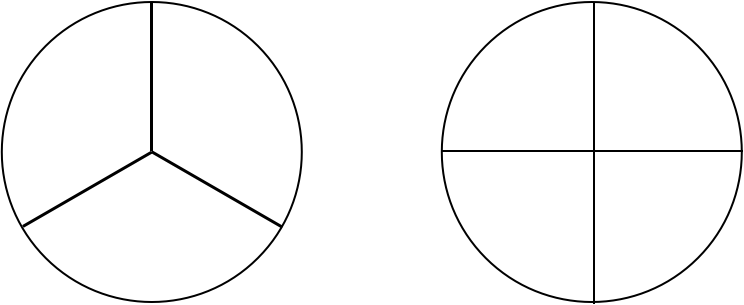
\includegraphics[scale=0.3]{FiguresMaths/AutomotiveBrands.png}
\end{center}
\caption{Idealized renditions of the logos on {\sc Mercedes}$^{\mbox{\tiny\sc tm}}$ (left) and BMW$^{\mbox{\tiny\sc tm}}$ (right) automobiles.}
\label{fig:auto-logos}
\end{figure}
The single-player {\it Logo game} proceeds as follows.  

\smallskip

Reflecting the fact that the {\sc Mercedes}$^{\mbox{\tiny\sc tm}}$ logo partitions the circle into {\em three} wedges, while the BMW$^{\mbox{\tiny\sc tm}}$ logo partitions the circle into {\em four} wedges, we assign the player---who, note, has not yet acted---with the initial scores
\[ M(0) \ = \ 3 \ \ \ \ \ \mbox{ and } \ \ \ \ \ B(0) = 4 \] 
and we designate the logo-circles in Fig.~\ref{fig:auto-logos} as the {\em stage-$0$} logo-circles.{\em Note that it is the {\em number} of wedges in each logo-circle that interests us, not the sizes of the wedges}.

The player now becomes active---
\medskip
************************************}

For each positive integer $k$, the player begins at the northernmost point of each stage-$(k-1)$ logo-circle and circumnavigates the circle in a clockwise sense.  In the course of this circumnavigation, the player {\em bisects every second wedge} that she encounters.  When the player regains the northernmost point of the two logo-circles, the numbers of wedges at that moment is recorded as the score at that moment, namely, the pair: at stage $k$ this has the form $\langle M(k), \ B(k) \rangle$. 
\medskip

{\em Prove the following assertions about the described game.}
\begin{itemize}
\item 3.
The asymptotic behavior of $B(n)$ is given by
\[ B(n) \ = \ \left({3 \over 2}\right)^{O(n)} \]
\end{itemize}



\medskip \item
{\bf 9.4. Karatsuba multiplication} 
\smallskip

\ignore{**************************
\index{Karatsuba multiplication algorithm} \index{Karatsuba, Anatoly} 
\index{Karatsuba multiplication}

{\sc Lesson:}
Use the Master Theorem for Linear Recurrences (Theorem~\ref{thm:master-thm-genl}) to analyze a recursive algorithm

\smallskip

Say that you are given two $n$-bit integers, in terms of their base-$2$ numerals: 
\[ A \ = \ a_{n-1} a_{n-2} \cdots a_0 \ \ \ \ \mbox{ and } \ \ \ \ B \ = \ b_{n-1} b_{n-2} \cdots b_0 \]
The classical elementary-school method for computing the product of $A$ and $B$ computes the $n$ partial products:
\[ (a_{n-1} a_{n-2} \cdots a_0) \times b_i 2^i \]
and then sums these partial products.  This algorithm requires $\Theta(n^2)$ multiplications and a like number of additions.

\smallskip

Now, multiplications are more expensive than additions on standard computing platforms.  Therefore, when the common length $n$ of the numerals for $A$ and $B$, is {\em very} large, then one would be willing to perform somewhat more additions (while staying within the asymptotic class $\Theta(n^2)$) if, in compensation, one could save a significant number of multiplications.  Happily, such a tradeoff is, indeed, available, using an algorithm that is known as {\it Karatsuba multiplication}, after its author, Anatoly Karatsuba; see \cite{KaratsubaO62}.

\medskip

Karatsuba's algorithm builds upon the {\it divide-and-conquer} algorithmic paradigm, whereby a
problem {\bf P} is decomposed into disjoint, equal-``size" subproblems whose results are accumulated to solve {\bf P}.
**************************}

The problem is to multiply two $n$-bit numerals $A$ and $B$.  
To simplify both notation and analysis, say that $n$ is a very large power of $2$, i.e., $n=2^k$ for some large $k \in \N^+$.
\smallskip

The algorithm breaks the numerals for $A$ and $B$ into pairs of half-size numerals:
\begin{eqnarray*}
A & = & A_1 \cdot 2^{n/2} \ + \ A_2 \ \ 
 \eqdef  \ \ (a_n \cdots a_{n/2+1})_2 \cdot 2^{n/2} \ + \ (a_{n/2} \cdots a_1)_2 \\
B & = & B_1 \cdot 2^{n/2} \ + \  B_2 \ \
  \eqdef  \ \ (b_n \cdots b_{n/2+1})_2 \cdot 2^{n/2} \ + \ (b_{n/2} \cdots b_1)_2
\end{eqnarray*}

{\em Prove the following assertions.}
\begin{enumerate}
\item 
{\em A recursion (on $n$) that is based on Karatsuba's algorithm computes the product $A \times B$ using {\em asymptotically fewer than} $\Theta(n^2)$ multiplications.}

\begin{equation}
\label{eq:karatsuba-normal}
A \times B \ = \ (A_1 \times B_1) \cdot 2^n \ + \  (A_1 \times B_2 \ + \ A_2 \times B_1) \cdot 2^{n/2} \ + \ (A_2 \times B_2)
\end{equation}

Let denote by $f(n)$ the cost for multiplying two $n$-bits numerals.
It is in $\Theta(n^2)$ in term of elementary bit- multiplications. 
The expression of $f$ is as follows:
\[
f(n) = \left\{
\begin{array}{cl}
4 f(n/2) + g(n) & \hspace*{.2in} \mbox{for } n > 1 \\
                    1 & \hspace*{.2in} \mbox{for } n = 1
\end{array}
\right. 
\]
where $g$ is the cost of the extra arithmetic operations done while merging the sub-problems. 
It corresponds to the two multiplications by powers of $2$ and three additions.
These additions are linear in $n$. Thus, $g(n) = \Theta(n)$

Applying the Master theorem gives the solution. 

\medskip
\item
Your argument should find a (real) number $\alpha < 2$ such that Karatsuba's algorithm computes the product $A \times B$ using $\Theta(n^\alpha)$ multiplications.
\smallskip

\[ C \ \eqdef \ (A_1 - A_2) \times (B_2 - B_1) \]
\begin{eqnarray*}
A \times B & = & (A_1 \times B_1) \cdot 2^n \ + \ (A_2 \times B_2) + \ \big(C \ + \ (A_1 \times B_1) \ + \ (A_2 \times B_2) \big) \cdot 2^{n/2}
\end{eqnarray*}

The cost analysis is 3 multiplications of $n/2$-bits numerals.
We performed 2 additions/subtractions of n-bits numerals for computing $C$ and
4 more additions. 
\[
f(n) = \left\{
\begin{array}{cl}
3 f(n/2) + \Theta(n) & \hspace*{.2in} \mbox{for } n > 1 \\
                    1 & \hspace*{.2in} \mbox{for } n = 1
\end{array}
\right. 
\]
Again, using the Master Theorem leads to:
$f(n) = 3^{\log_2 n} = n^{\log_2 3}$

$\alpha = \log_2 3 < 2$
\end{enumerate}

\end{itemize}


%
%\subsection{Solving a bilinear recurrence by a linear system}
%
%\noindent 
%The goal here is to determine the values of  $U_n$
%
%Solve $U_{n} = \frac{1}{2}.U_{n-1} + \frac{1}{2}.U_{n+1}$
%
%knowing $U_0 = 0$ and $U_N = 1$
%



\ignore{
*****\subsection{Lucas' numbers}

\noindent \textit{The problem.}

Prove the following expression.
 
$F(n+1) = \frac{1}{2} (F(0).L(n) + F(n).L(0))$
\medskip

\noindent \textit{The solution.}
The proof comes from direct arithmetic manipulations:

$2.F(n+1) = F(n+1) +  F(n+1) =  F(n+1) + F(n) + F(n-1)$

$= L(n) + F(n) $

$= F(0).L(n) + F(n).L(0)$
\medskip

\noindent \textit{The problem.}

The previous property can be extended for any $m>1$ as follows:
\medskip

$2.F(n+m) = F(m-1).L(n) + F(n).L(m-1)$
\medskip

\noindent \textit{The solution.}
The proof is by recurrence on $m$ considering any fixed $n$.
\begin{itemize}
\item
The \textbf{basis case} (for $m=1$) is given by the previous proposition.

\item
\textbf{Induction step:} 
Assume the property holds at rank $m > 1$ and consider $F(n+m+1)$:

Apply the definition of Fibonacci numbers: 

$F(n+m+1) = F(n+m)+F(n+m-1)$ 

Replace both terms by the recurrence hypothesis:

$= \frac{1}{2} (F(m-1).L(n) + F(n).L(m-1)) + \frac{1}{2} (F(m-2).L(n) + F(n).L(m-2))$

$= \frac{1}{2} \left( (F(m-1)+F(m-2)).L(n) + F(n).(L(m-1)+L(m-2))\right)$

$= \frac{1}{2} \left(F(m).L(n) + F(n).(L(m)\right)$
\end{itemize}
***** }

%%%%%%%%%%%%%%%%%%%%%%%%%%%%%%%%%%%%%%%%%

%\section*{Exercises: Chapter 10}

\ignore{***************************************
\subsection{The average length of a carry in a binary counter}

\noindent {\it The problem.}
%
You add from $1$ to $n$, in increments of $1$ using a counter of
binary (or, base-$2$) numerals.  Each time you increment the counter,
there is a {\it carry}.  These carries have varying lengths; for
instance, when $n = 32 = 100000_2$, the carry-lengths range
from $0$---whenever you increment an even integer---to $5$---when you
increment $31 = 11111_2$ to achieve $32 = 100000_2$. \\
{\em Prove that the average carry as you go from $1$ to $n$ has length $2$.}
\medskip

\noindent {\it The solution.}

\noindent
Half of the increments add $1$ to an even number, i.e., a number whose
binary numeral ends in ``$ \ldots 0$''.  These increments generate no
carry---or, equivalently, a carry of length $0$.

\noindent
One-quarter of the increments, which form half of the remaining
increments, execute a carry of length $1$, because they add $1$ to a
numeral that ends in ``$ \ldots 01$''.

\noindent
One-eighth of the increments, which form half of the remaining
increments, execute a carry of length $2$, because they add $1$ to a
numeral that ends in ``$ \ldots 011$''.

Continuing in this way, one can show that the average length of a
carry can be expressed in the form
\[ 
\frac{1}{2} \cdot 0 \ + \ \frac{1}{4} \cdot 1 \ + \ \frac{1}{8} \cdot
3 \ + \ \frac{1}{16} \cdot 4 \ + \ \cdots
\]
Using techniques that we cover in Chapter~\ref{ch:Summation}, one
verifies that this infinite series converges with the sum $2$.  \qed
********************************}

\begin{itemize}

\item
{\bf 10.3. The Josephus Problem}
\medskip

 Fig~\ref{fig:josephus12step1} and Fig.~\ref{fig:josephus12step2} describe pictorially the rounds of the Josephus process
 for determining the survivor number $J(n)$.
\begin{figure}[ht]
\begin{center}
        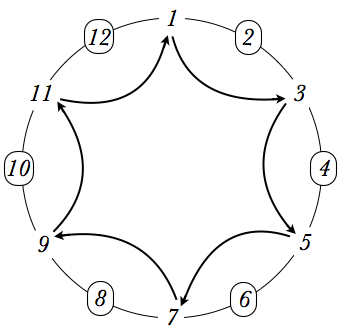
\includegraphics[scale=0.3]{FiguresMaths/josephus12step1}
\caption{First round of the Josephus erasure process for $n=12$. The circled numbers are those that are removed.}
        \label{fig:josephus12step1} 
%\end{center}
%\end{figure}
%\begin{figure}[ht]
%\begin{center}
        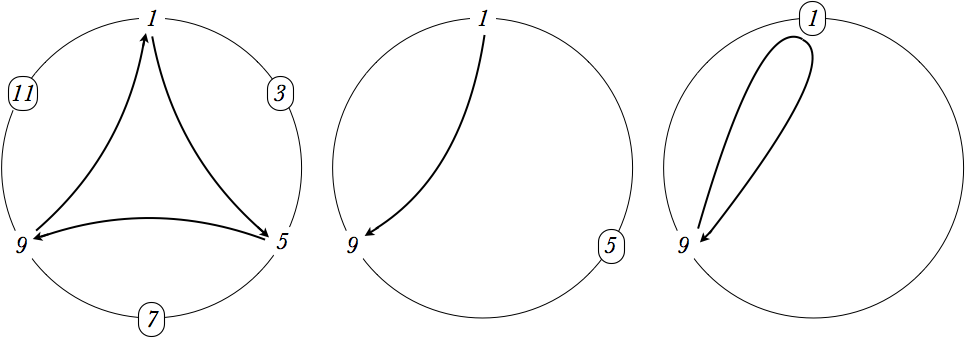
\includegraphics[scale=0.3]{FiguresMaths/josephus12LastSteps}
        \caption{The final rounds of the Josephus process when $n=12$ leading to $J(12) = 9$}
        \label{fig:josephus12step2}
\end{center}
\end{figure}

The following sequence of results provide a roadmap to the solution.

\medskip
%
%We analyze \textit{rounds} of the process---sequences of elementary steps that return to the initial position, $1$.  If position $1$ has been erased, then its role is assumed by the then-smallest survivor.
%\smallskip

The first round of the process takes $\lceil n/2 \rceil$ steps.  
Each subsequent round then takes a number of steps that is ``half" the number of its preceding round.  We place ``half" in quotes to emphasize the required up-rounding of each halving.  
\medskip

{\em Prove the following quadripartite proposition 
that provides a characterization of $J(n)$ for some particular values of $n$.

\begin{tabular}{clll}
 & \underline{Condition on $n$} & \hspace*{.1in} & \underline{Value of $J(n)$} \\ 
{\bf (a)} &
For all $n$ &  & $J(n)$ is odd. \\
{\bf (b)} &
$n$ is even; i.e., $n = 2m$ & & $J(2m) = 2J(m)-1$ \\
{\bf (c)} &
$n$ is odd; i.e., $n = 2m+1$ & & $J(2m+1) = 2J(m)+1$ \\
{\bf (d)} &
$n = 2^m+k$, with $k < 2^m$ & & $J(2^m+k) = 2k+1$
\end{tabular}
}

\begin{proof}
\begin{itemize}
\item {\bf (a)} 
All the even numbers are removed from the circle at the first round, thus, it remains only odd numbers.
\medskip

\item {\bf (b)} 
is a simple generalization of {\bf a}.  
If $n$ is even, then the first round corresponds to come back to the original circle 
where one half of the points have been removed. 
In other words, rank $i$ becomes rank $(2.i-1)$.
\medskip

\item {\bf (c)} 
is the counter part of {\bf b} for the odd numbers.

\item {\bf (d)} 
Observing the successive values for small $n$ evidences that the $J(n)$ are grouped by successive powers of $2^m$
and the rule within each group is to start at $1$ and then, increase by $2$ the successive numbers until reaching the next group
($0 \leq k < 2^m$).

Formally, the proof of $J(2^m+k) = 2k+1$ is by recurrence on $n$.

\noindent
{\sf Base}.
$n=1$, thus $m=0$, $k=0$ and $J(1) = 2^0+0 = 1$
\smallskip

\noindent 
{\sf Inductive hypothesis}.
Suppose the formula holds for any integer lower than $n=2^m+k$.
\smallskip

\noindent 
{\sf Inductive extension}.
Since there are two expressions for $J(.)$, we distinguish the cases whether $k$ is even or if it is odd:
\begin{itemize}
\item If $k$ is even, then, $2^m+k$ is even, and we can write:

$J(2^m+k) = 2.J(2^{m-1}+\frac{k}{2})-1$

by induction hypothesis, $J(2^{m-1} +\frac{k}{2}) = 2\frac{k}{2} +1 = k+1$

Thus, $J(2^m+k) = 2(k+1) -1 = 2k+1$.

\item 
If $k$ is odd, the proof is similar:

$J(2^m+k) = 2J(2^{m-1}+\lfloor \frac{k}{2} \rfloor)+1 = 2\lfloor \frac{k}{2} \rfloor +1 = 2k+1$.
\end{itemize}

\end{itemize}
\end{proof}

Your ultimate solution for $J(n)$ will emerge from analyzing what the preceding propositions yield as the value of $J(n)$.  

{\em Provide a closed-form expression for $J(n)$ in terms of $n$'s base-$2$ numeral.}
\medskip

Consider the binary {\em numerals} for $n = 2^m +k$ and $k$.  We first note that, {\em numerically},
\begin{eqnarray*}
n & = &  2^m b_m \ + \ 2^{m-1} b_{m-1} \ + \cdots + \ 2 b_1 \ + \ b_0 \\
k & = & 2^{m-1}  b_{m-1} \ + \cdots + \ 2 b_1 \ + \ b_0
\end{eqnarray*} 
where each bit $b_i \in \{0,1\}$.  Therefore, in terms of {\em base-$2$ numerals}:
\[ \begin{array}{ccrl}
(n)_2 & = & 1 b_{m-1} \cdots b_1 b_0 & (\mbox{by definition, } \ b_m=1) \\ 
(k)_2 & = & 0 b_{m-1} \cdots b_1 b_0 & (\mbox{because } [n = 2^m +k] \ \mbox{ and } \ k < 2^m)
\end{array}
\]

\[ (J(n))_2 \ = \ b_{m-1} \cdots b_0 b_m. \]
The solution for $J(n)$ is obtained by a simple shift to the left of the binary representation of $n$
with a $1$ at the rightmost position.
The pictorial interpretation of this coding is given in Fig.~\ref{fig:josephusCoding} for $n=43$.
\begin{figure}[h]
\begin{center}
        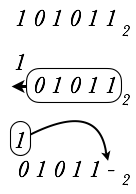
\includegraphics[scale=0.4]{FiguresMaths/josephusCoding}
        \caption{Obtaining the survivor number $J(43)=23$.}
        \label{fig:josephusCoding}
\end{center}
\end{figure}

\end{itemize}

%%%

\begin{itemize}
\item {\bf 10.5. An alternative to Horner's Rule}

\smallskip

%In Section~\ref{sec:Horner-fast-evaluation}, we described Horner's Rule, a method for calculating polynomials faster than the common way of writing polynomials would suggest.  This exercise is devoted to an alternative streamlined polynomial evaluation procedure, called {\it Estrin's method}, after its inventor, Gerald Estrin \cite{Estrin60}.
%\smallskip

Estrin's method begins with a polynomial of degree $d$ with real coefficients:
\[
P(x) \ \ = \ \ a_0 \ + \ a_1 x \ + \ a_2 x^2 \ + \cdots + \ a_{d-1} x^{d-1} \ + \ a_d x^d
\]
which is transformed as follows:
\[
P(x) \ \ = \ \ a_0 \ + \ x \cdot (a_1 \ + \ x \cdot (a_2  \ +  \cdots                                          
+ x \cdot (a_{d-2} \ + \ x \cdot (a_{d-1} \ + \ a_d x)) \cdots ))
\]
%To avoid complicated expressions, we apply the method to the degree-$(d=7)$ polynomial:
%\[
%P_7(x) \ \ = \ \ a_0 \ + \ a_1 x \ + \ a_2 x^2 \ + \ a_3 x^3 \ + \ a_4 x^4 \ + \ a_5 x^5 \ + \ a_6 x^6 \ + \ a_7 x^7
%\]
%\[
%P_7(x) \ \ = \ \ a_0 \ + \ a_1 x \ + \ x^2 \ ( a_2  \ + a_3 x \ ) \ + \ x^4 \ ( \ a_4 \ + \ a_5 x \ + \ x^2 \ ( a_6  \ + a_7 x \ ) \ )
%\]
We then introduce the recursively auxiliary expressions.  
\begin{eqnarray*}
C_i^{(0)} & = & a_i + x a_{i+1} \\
                &\vdots &  \\
C_i^{(n)}  & = & C_i^{(n-1)} + x^{2n} C_{i+2^n}^{(n-1)}
\end{eqnarray*}
The method completes by expressing $P(x)$ in terms of the auxiliary $C_i^{(k)}$
\smallskip

Example (for a degree-$(d=7)$ polynomial):
\begin{eqnarray*}
P_7(x) & = & C_{0}^{(0)} \ + \ x^2 \ C_2^{(0)} \ + \ x^4 \ ( \ C_4^{(0)} \ + \ x^2 \ C_6^{(0} \ )
\end{eqnarray*}
\medskip

\begin{enumerate}
\item
{\em Write $P(x)$ using the auxiliary expressions $C_i$.}  
We consider that $d+1$ is a power of $2$.
\begin{eqnarray*}
P_7(x)            & = & C_0^{(1)} \ + \ x^4 \ C_4^{(1)}
\end{eqnarray*}

\item
{\em Determine how many additions and multiplications are required to evaluate $P(x)$.}

Let study this question in detail for $d=7$.
\[
P_7(x) \ \ = \ \ C_{0}^{(0)} \ + \ x^2 \ C_2^{(0)} \ + 
\ x^4 \ ( \ C_4^{(0)} \ + \ x^2 \ C_6^{(0} \ )
\ = \ C_0^{(1)} \ + \ x^4 \ C_4^{(1)} 
\]
There are $2$ multiplications for computing $x^2$ and $x^4$

Then, 4 multiplications by $x$ for the products $a_7 x$,  $a_5 x$, $a_3 x$ and $a_1 x$
followed by 4 additions.

2 multiplications by $x^2$ for $x^2 C_2^{(0)}$ and $x^2 C_6^{(0)}$
followed by 2 additions

Finally, 1 multiplication for computing $x^4 C_4^{(1)}$
followed by 1 addition
\medskip

Total of $2 + 7$ multiplications and $7$ additions.
\medskip

Generalization: 
$\Theta(d + log_2(d))$ multiplications and $\Theta(d)$ additions.
\end{enumerate}
\end{itemize}


%%%%%%%%%%%%%%%%%%%%%%%%%%%%%%%%%%%%%%%%%
% \section{Chapter 11}
\begin{itemize}
\item
{\bf 11.2. Counting replicated triangles}
\smallskip

{\em How does the progression of numbers of triangles contained into the rank $k$ triangle $T_k$ grow?}
Let $N_k$ denote this number of triangles within $T_k$.  
We know that $N_0 =1$, $N_1 = 5$, and $N_2 = 13$.
  \begin{enumerate}
  \item
{\em Compute} $N_4$.
\smallskip

First, let remark that there is only one large triangle $T_4$.

$T_4$ is represented in Fig.~\ref{fig:countingTriangles3} where there are clearly $3$ triangles $T_3$
that partially overlap.
\begin{figure}[h]
\begin{center}
        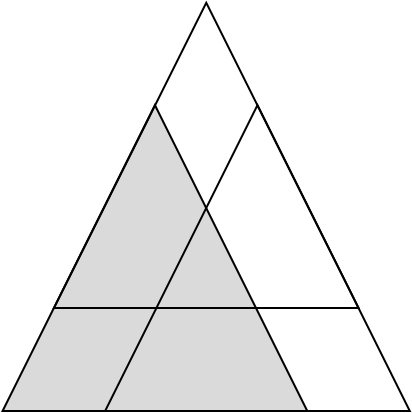
\includegraphics[scale=0.3]{FiguresArithmetic/CountingTriangles3} 
        \caption{The $3$ triangles $T_3$ contained into $T_4$.}
        \label{fig:countingTriangles3}
\end{center}
\end{figure}
Let us now enumerate the $T_2$ triangles
(see Fig.~\ref{fig:countingTriangles2}).
\begin{figure}[h]
\begin{center}
        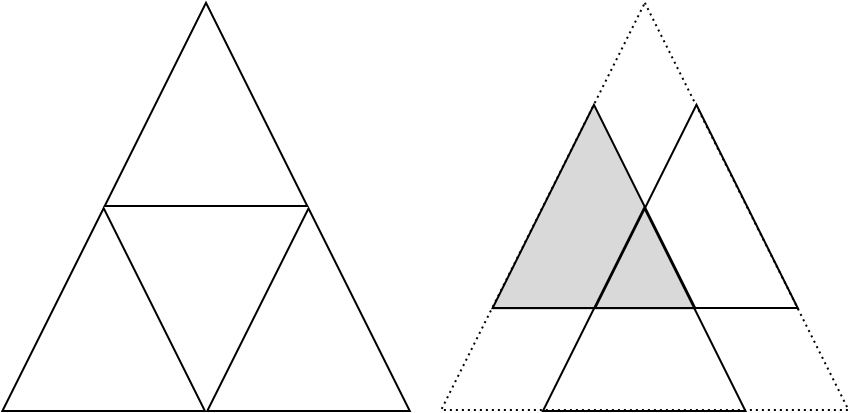
\includegraphics[scale=0.3]{FiguresArithmetic/CountingTriangles2} 
        \caption{$4$ triangles $T_2$(left) and $3$ triangles $T_2$(right).}
        \label{fig:countingTriangles2}
\end{center}
\end{figure}
Let us now jump to the smallest $T_1$.
Counting them row by row indicates that their number is equal to the sum of the first $k$ integers (here $k=4$).
This sum is well-known and it is equal to the square of the rank: $4^2 = 16$.
\smallskip

Summing up all levels, we obtain:

$N_4 = 1 + 3 + 7 + 16 = 27$.

\medskip\item
{\em Develop a recurrence for} $N_k$ (i.e., the general case).
\smallskip

The recurrence is based on the generalization of the analysis of the previous case $k=4$.

For each triangle $T_k$, we have $3$ intertwined triangles $T_{k-1}$ (thus, $3 N_{k-1}$).
Two of these triangles share a common part, this part is a triangle $T_{k-2}$ that should be removed from the counting
(which corresponds to $ -3 N_{k-2}$).
But there is another part which is common to these three triangles. This part is a lower dimension $T_{k-3}$ (thus, $+ N_{k-3}$). 
Finally, we should add the largest triangle $T_{k}$ (this corresponds to $+1$), and when $k$ is even,  there is an extra triangle $T_{k-2}$ that
appears reversed in the middle (therefore, we should add $+1$ in this case).
\smallskip

The summary is as follows:

For even $k$:  $N_k = 3 (N_{k-1} - N_{k-2}) + N_{k-3} + 1 + 1$

For odd $k$: $N_k = 3 (N_{k-1} - N_{k-2}) + N_{k-3} + 1$

with $k \geq 3$ et $N_0 = 0$, $N_1 = 1$ et $N_2 = 5$\footnote{We added the artificial case $k=0$ in order to simplify the expression}.
\medskip

The most discerning readers may check that solving this recurrence leads to the following expression:

$N_k = \frac{k.(k+2).(2k+1)}{8}$ if $k$ is even

$N_k = \frac{k.(k+2).(2k+1)-1}{8}$ if $k$ is odd.
\end{enumerate}

%%%


\medskip\item
{\bf 11.6. Monge shuffles: mathematical party tricks}
\smallskip

For both shuffle-techniques. we begin with a deck of $2n$ distinct cards.  
We employ the running example of the following small deck, where $n=4$:
\[ (1, \ 2, \ 3, \ 4, \ 5, \ 6, \ 7, \ 8) \]
For both {\it Monge shuffles} of the cards, we cut the deck in the middle, to create two $n$-card decks:
\[ (1, \ 2, \ 3, \ 4), \ (5, \ 6, \ 7, \ 8) \]
We then merge the two $n$-card decks to again obtain a single $2n$-card deck.  The two Monge shuffles differ in their merging techniques.

  \begin{enumerate}
  \item $\oplus$ {\bf The simple Monge shuffle}

\smallskip

The first, simple, Monge shuffle alternates the ``top" cards from the righthand and lefthand $n$-card decks; see Fig~\ref{fig:suffleMonge}.  The merged deck has the form
\[ (5, \ 1, \ 6, \ 2, \ 7, \ 3, \ 8, \ 4) \]
\begin{figure}[h]
\begin{center}
        \includegraphics[scale=0.4]{FiguresArithmetic/suffleMongeBasic}
        \caption{The Monge shuffle for $8$ cards ($n=4$).}
        \label{fig:suffleMonge}
\end{center}
\end{figure}

In the party-game incarnation of the Monge shuffle, you demonstrate the cut-then-merge process of Fig~\ref{fig:suffleMonge}, and you suggest to your audience that this process is a good first step in really mixing up the cards.  If this were so, then repeating the step several times should be a good way to obtain a ``random" mixture of the cards.

\smallskip

Let's see what happens after several steps of this cut-then-merge process:
\[ \begin{array}{ccccccccccccccccc}
(1 & 2 & 3 & 4 & 5 & 6 & 7 & 8) & \rightarrow & (1 & 2 & 3 & 4) & (5 & 6 & 7 & 8) \\
 & & & & & & & & \swarrow & & & & & & & & \\
(5 & 1 & 6 & 2 & 7 & 3 & 8 & 4) & \rightarrow & (5 & 1 & 6 & 2) & (7 & 3 & 8 & 4) \\
 & & & & & & & & \swarrow & & & & & & & & \\
(7 & 5 & 3 & 1 & 8 & 6 & 4 & 2) &  \rightarrow& (7 & 5 & 3 & 1) & (8 & 6 & 4 & 2) \\
 & & & & & & & & \swarrow & & & & & & & & \\
(8 & 7 & 6 & 5 & 4 & 3 & 2 & 1) &  \rightarrow& (8 & 7 & 6 & 5) & (4 & 3 & 2 & 1) \\
 & & & & & & & & \swarrow & & & & & & & & \\
(4 & 8 & 3 & 7 & 2 & 6 & 1 & 5) &  \rightarrow& (4 & 8 & 3 & 7) & (2 & 6 & 1 & 5) \\
 & & & & & & & & \swarrow & & & & & & & & \\
(2 & 4 & 6 & 8 & 1 & 3 & 5 & 7) &  \rightarrow& (2 & 4 & 6 & 8) & (1 & 3 & 5 & 7) \\
 & & & & & & & & \swarrow & & & & & & & & \\
(1 & 2 & 3 & 4 & 5 & 6 & 7 & 8)
\end{array}
\]
So, this does not look too random!  After {\em three} (which, ``coincidentally", equals $n-1$) cut-then-merge steps, the deck has been reversed, and after $2n-1$ cut-and-merge steps, it has been replicated in its original order!
\medskip

{\em Prove the following Proposition.}

Let $p$ be a prime ($p>2$), and let $n = {1 \over 2} (p-1)$.  
Let us begin with a deck of $2n$ distinct cards and perform the simple Monge shuffle on the deck.  
After some number $m$ of cut-then-merge steps, where $m$ divides $p-1$, the simple Monge shuffle replicates the initial deck.
\smallskip

Studying our sample sequence of cut-then-merge steps should provide a valuable hint.

\medskip
\item {\bf The sophisticated Monge shuffle}
\smallskip

We now provide a more sophisticated merge procedure, which yields a sophisticated variant of the Monge shuffle.  In each stage of this variant---each corresponding to a cut-then-merge step of the simple shuffle---we rearrange the $2n$-card deck directly, from the middle outward, via the following regimen:

\smallskip

\noindent
- Card \#1 of the original deck is placed in position $n+1$ of the shuffled deck \\
- Card \#2 of the original deck is placed in position $n$ of the shuffled deck \\
- Card \#3 of the original deck is placed in position $n+2$ of the shuffled deck \\
- Card \#4 of the original deck is placed in position $n-1$ of the shuffled deck \\
\hspace*{.1in} \ldots and so on, until the original deck is empty.

\smallskip
\ignore{********************************
The first few steps of a stage of the sophisticated Monge shuffle are illustrated for the case $n=4$ in Fig.~\ref{fig:suffleMonge1};
\begin{figure}[h]
\begin{center}
        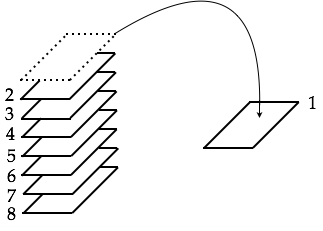
\includegraphics[scale=0.33]{FiguresArithmetic/suffleMongeStep1}
        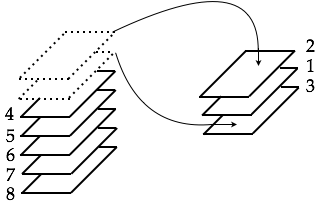
\includegraphics[scale=0.33]{FiguresArithmetic/suffleMongeStep2}
         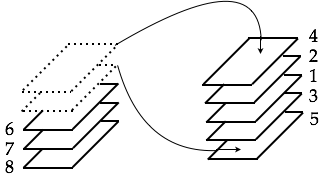
\includegraphics[scale=0.33]{FiguresArithmetic/suffleMongeStep3}
        \caption{The Monge shuffle for $8$ cards ($n=4$): Step 1 (left), Step 2 (center), Step 3 (right).}
        \label{fig:suffleMonge1}
\end{center}
\end{figure}
one complete stage is illustrated in the table following the figure.
\[ \begin{array}{cccccccccccccccccc}
\mbox{Step } & \multicolumn{8}{c}{\mbox{Original deck}} & &
     \multicolumn{8}{c}{\mbox{Shuffled deck}} \\
\hline
1 & (1 & 2 & 3 & 4 & 5 & 6 & 7 & 8) & \rightarrow & ( - & - & - & - & 1 & - &  - & - ) \\
2 & ( - & 2 & 3 & 4 & 5 & 6 & 7 & 8) & \rightarrow & ( - & - & - & 2 & 1 & - & - & - ) \\
3 & ( - & - & 3 & 4 & 5 & 6 & 7 & 8) &  \rightarrow& ( - & - & - & 2 & 1 & 3 & - & - ) \\
4 & ( - & - & - & 4 & 5 & 6 & 7 & 8) &  \rightarrow& ( - & - & 4 & 2 & 1 & 3 & - & - ) \\
5 & ( - & - & - & - & 5 & 6 & 7 & 8) &  \rightarrow& ( - & - & 4 & 2 & 1 & 3 & 5 & - ) \\
6 & ( - & - & - & - & - & 6 & 7 & 8) &  \rightarrow& ( - & 6 & 4 & 2 & 1 & 3 & 5 & - ) \\
7 & ( - & - & - & - & - & - & 7 & 8) &  \rightarrow& ( - & 6 & 4 & 2 & 1 & 3 & 5 & 7 ) \\
8 & ( - & - & - & - & - & - & - & 8) &  \rightarrow& ( 8 & 6 & 4 & 2 & 1 & 3 & 5 & 7 ) \\
\end{array}
\]
*********************************}

\medskip

{\em Prove the following Proposition.}

For any integer $n \in \N^+$: 
If $4n+1$ is prime, then performing $2n$ steps of the sophisticated Monge shuffle on a deck of $2n$ distinct cards restores the deck to its original order.
\end{enumerate}
  
\end{itemize}


%%%%%%%%%%%%%%%%%%%%%%%%%%%%%%%%%%%

%\section*{Exercises: Chapter 12}

\ignore{******************************************
\subsection{Formal definition of mesh graphs}
\label{Exercice:FormalDefinitionMesh}

\noindent \textit{The problem.}
Formalize precisely the definition of mesh  $\m_{m,n}$ and torus $\widetilde{\m}_{m,n}$ graphs
for positive integers $m, n \in \N^+$.
\medskip

\noindent \textit{The solution.}
The  {\it vertex-set} is the same for both graphs:

\begin{eqnarray*}
\n_{\fm_{m,n}} \ = \ \n_{\widetilde{\fm}_{m,n}}
  & = & 
\{1, \ 2, \ldots, \ m\} \ \times \ \{1, \ 2, \ldots, \ n\} \\
  & = & 
\big\{ \langle i, \ j \rangle \ \ | \ \ 
\big[ i \in \{1, \ 2, \ldots, \ m\} \big], \ \
\big[ j \in \{1, \ 2, \ldots, \ n\} \big]
\big\}
\end{eqnarray*}

$\m_{m,n}$ has $(m-1)n \ + \ (n-1)m$ edges; its {\it edge-set} is
\begin{eqnarray*}
\e_{\fm_{m,n}} & = & 
\big\{
\{ \{ i, j \}, \ \{ i+1, j \} \ \ | \ \
1 \leq i < m, \ \ 1 \leq j \leq n \} \\
  &  & \hspace*{.1in} \cup
\{ \{ i, j \}, \ \{ i, j+1 \} \ \ | \ \
1 \leq i \leq m, \ \ 1 \leq j < n \}
\big\}
\end{eqnarray*}

\medskip

The subgraph of $\m_{m,n}$ defined by the vertex-set
\[ \{ \langle i, \ j \rangle  \ \ | \ \ \left[i \in \{1, 2, \ldots,
  m\}\right], \ \ \left[1 \leq j < n\right]\}
\]
and all edges both of whose endpoints belong to that set is called the
$i$th {\it row} of $\m_{m,n}$
Dually, the subgraph of $\m_{m,n}$ defined by the vertex-set
\[ \{ \langle i, \ j \rangle  \ \ | \ \ \left[j \in \{1, 2, \ldots,
  n\}\right], \ \ \left[1 \leq i < m\right] \}
\]
and all edges both of whose endpoints belong to that set is called the
$j$th {\it column} of $\m_{m,n}$.


\begin{itemize}
     \item
Vertices $\langle 1, \ 1 \rangle$, $\langle 1, \ n \rangle$, $\langle m,
\ 1 \rangle$, and $\langle m, \ n \rangle$ are the {\it corner vertices}
(or, just {\it corners}) of $\m_{m,n}$.
     \item
The path-graph consisting of the vertex-set
\[ \{ \langle 1, \ 1 \rangle, \ \langle 1, \ 2 \rangle, \ldots, \
\langle 1, \ n \rangle \}
\]
together with all edges of $\m_{m,n}$ both of whose endpoints belong
to this set, is the {\it top edge} of $\m_{m,n}$.

The other edges of $\m_n$ are defined analogously:

\medskip

The {\it bottom edge} of $\m_{m,n}$ is the path-graph built upon the
vertex-set
\[ \{ \langle m, \ 1 \rangle, \ \langle m, \ 2 \rangle, \ldots, \
\langle m, \ n \rangle \}
\]

The {\it left edge} of $\m_{m,n}$ is the path-graph built upon the
vertex-set
\[ \{ \langle 1, \ 1 \rangle, \ \langle 2, \ 1 \rangle, \ldots, \
\langle m, \ 1 \rangle \}
\]

The {\it right edge} of $\m_{m,n}$ is the path-graph built upon the
vertex-set
\[ \{ \langle 1, \ n \rangle, \ \langle 2, \ n \rangle, \ldots, \
\langle m, \ n \rangle \}
\]
\end{itemize}
\medskip

Same for the torus graphs:

The subgraph of $\widetilde{\m}_{m,n}$ defined by the vertex-set
\[ \{ \langle i, \ j \rangle  \ \ | \ \ \left[i \in \{1, 2, \ldots,
  m\}\right], \ \ \left[1 \leq j \leq n\right]\}
\]
and all edges both of whose endpoints belong to that set is called the
$i$th {\it row} of $\widetilde{\m}_{m,n}$
Dually, the subgraph of$\widetilde{\m}_{m,n}$ defined by the vertex-set
\[ \{ \langle i, \ j \rangle  \ \ | \ \ \left[j \in \{1, 2, \ldots,
  n\}\right], \ \ \left[1 \leq i \leq m\right] \}
\]
and all edges both of whose endpoints belong to that set is called the
$j$th {\it column} of $\widetilde{\m}_{m,n}$.
%\medskip
%
%\noindent \textit{Lesson learned.}
%manipulate mathematical symbols. 
****************************************}

\begin{itemize}
\item
{\bf 12.1. Vertex-degrees and the existence of paths}
\smallskip

{\em Prove that if every vertex of graph $\g$ has degree $\geq d$, then $\g$ contains a {\em simple} path of length $d$.}
\smallskip

Let us consider a \textit{maximal} path in $\g$ (that is a path of maximum length). 

Take an extremity of this path, we denote by $x$ this vertex.
As the path is maximal, all the vertices adjacent to $x$ belong to this path (otherwise, the path will be increased
and it contradicts the maximality).

Every vertices, including $x$, have a degree more than $d$, thus, the path has at least $d$ other vertices.

\medskip\item
{\bf 12.2. Vertex-degrees and their distributions in graphs}
\smallskip

{\em Prove the following results.}

\begin{prop}
Let $\g$ be an arbitrary graph.
\smallskip

\noindent
{\bf (a)} The sum of $\g$'s vertex-degrees is even.
\smallskip

\noindent {\bf (b)}
The number of $\g$'s vertices having odd vertex-degree is even.
\end{prop}

\medskip\item
{\bf 12.8. A small graph isomorphism}
\smallskip

{\em Prove the following Proposition:}
\smallskip

{\em The order-$4$ hypercube $\q_4$ is \textit{isomorphic} to the $4 \times 4$ torus $\widetilde{\m}_{4,4}$.}
\smallskip

%Try to find a relation (an ``encoding") between the bit-strings that name the vertices of $\q_4$ and the ordered pairs of integers that name the vertices of $\widetilde{\m}_{4,4}$.
%\smallskip 
%
%Once you get an idea for how such an ``encoding" might work, try to incorporate the inter-vertex names of edges for both graphs.
%\medskip

$\q_4$ is represented by its natural Gray codes,
where a vertex is coded 4 bits and connected to its four neighbors by complementing 
the digit in each of the four dimensions.
Fig.~\ref{fig:IsomorphismCodingPrinciple}(left) depicts this coding of a vertex and its neighbors.
\medskip

$\widetilde{\m}_{4,4}$ is the cartesian product between two cycles.
Each one is composed of the four vertices connected using the Gray code
$00, 01, 11, 10$.
Fig.~\ref{fig:IsomorphismCodingPrinciple}(right) shows this coding and 
its correspondence with the hypercube. 
The whole coding is obtained by concatenation of both dimensions (horizontal and vertical).
See Fig.~\ref{fig:IsomorphismCodingComplete}
For instance the bottom left vertex is $00 | 00$. 
\medskip
 \begin{figure}[hbt]
\begin{center}
       \includegraphics[scale=0.4]{FiguresGraph/IsomorphismEx2}
       \caption{Coding schemes for the hypercube and torus.}
  \label{fig:IsomorphismCodingPrinciple}
\end{center}
\end{figure}
 \begin{figure}[hbt]
\begin{center}
       \includegraphics[scale=0.4]{FiguresGraph/IsomorphismEx1}
       \caption{Complete coding schemes.}
  \label{fig:IsomorphismCodingComplete}
\end{center}
\end{figure}

The above description of the codings shows the one-to-one correspondence between the vertices of each graph.
The next step is to show the one-to-one correspondence of the relative edges.


\medskip\item
{\bf 12.9. A traffic map for a mesh-structured city}
\smallskip

%Here is a {\em highly structured, recursive} proposal for a traffic network.  To simplify our work, let us assume that $N$ has the form $n^2$ with $n = 2^{m}$. 
%  \begin{itemize}
%  \item
%We logically arrange the city's $N$ sites in an $n \times n$ grid by assigning each site a distinct name of the form $\langle i,j \rangle$, where $i, j \in \{1, 2, \ldots, n\}$.
%
%\smallskip
%Fig.~ \ref{fig:routingCity} gives an illustration of the previous textual description.
%\begin{figure}[hbt]
%\begin{center}
%       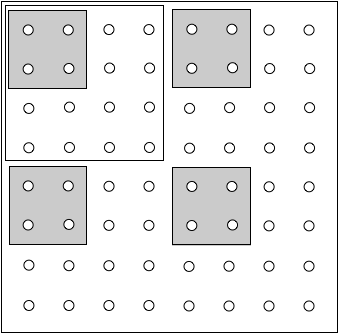
\includegraphics[scale=0.4]{FiguresGraph/routingCity}
%\caption{A $64$-site city arranged as an $8 \times 8$ grid.  The figure illustrates: the level-$0$ $8 \times 8$ grid and its northwestern $4 \times 4$ quadrant; the grid's four level-$2$ northwestern $2 \times 2$ quadrants (shaded).}
%  \label{fig:routingCity}
%\end{center}
%\end{figure}
%\begin{figure}[hbt]
%\begin{center}
%       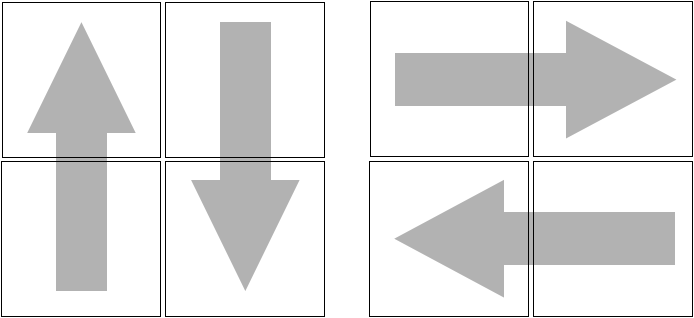
\includegraphics[scale=0.3]{FiguresGraph/routingCitySynthesis}
%\caption{Summary of the routing rules.}
%  \label{fig:routingCitySynthesis}
%\end{center}
%\end{figure}
%  \medskip\item
%We turn now to the (oriented) edges that we use to navigate our grid-like city.
%
%\smallskip
%
%We eliminate (from consideration) all ``diagonal" edges.  Phrased positively: we employ only edges whose endpoint-sites share a coordinate.  Each of these edges goes from a site $\langle i,j \rangle$ to a site $\langle i,k \rangle$ or a site $\langle h,j \rangle$.
%
%\smallskip
%
%This means that every {\em oriented} edge now goes either northward or southward or eastward or westward.
%
%\medskip\item
%We now assign (oriented) edges to levels, as a prelude to our routing regimen.
%
%\smallskip
%
%Focus on an edge $e$.  We say that $e$ is a level-$\ell$ edge if $\ell$ is the smallest integer such that the endpoints of $e$ are in distinct level-$\ell$ quadrants.
%
%  \medskip\item
%As the final step in creating our abstract traffic model, we impose the following routing regimen upon the travelers in our city.
%
%\smallskip
%
%In order to travel from site $\langle i,j \rangle$ to site $\langle h,k \rangle$, a traveler:
%    \begin{itemize}
%    \item
%must traverse the at-most three edges that lead site $\langle i,j \rangle$ to some site $\langle i_1,j_1 \rangle$ within the same quadrant as site $\langle h,k \rangle$.
%
%   \medskip\item
%From that point on, the traveler recursively finds an acceptable path from site $\langle i_1,j_1 \rangle$ to site $\langle h,k \rangle$.
%    \end{itemize}
%  \end{itemize}

In both of the sought analyses, the phrase ``worst-case" means that the sites are situated pessimally for our regimen.
  \begin{enumerate}
  \item
In the {\em metro} version of the model, we pay a fee every time we encounter a new site on the way from $\langle i,j \rangle$ to $\langle h,k \rangle$.

\smallskip

{\em What is the cost of a trip from a site $\langle i,j \rangle$ to the most-distant site,$\langle h,k \rangle$, under the \underline{metro} model?}

  \medskip\item
In the {\em driving} version of the model, we pay a per-kilometer fee of $n^{(1/2)^\ell}$ units every time we traverse a level-$\ell$ edge on the way from $\langle i,j \rangle$ to $\langle h,k \rangle$.
 
 \smallskip

{\em What is the cost of a trip from a site $\langle i,j \rangle$ to the most-distant site, $\langle h,k \rangle$, under the \underline{driving} model?}

 \end{enumerate}
 \begin{figure}[hbt]
\begin{center}
       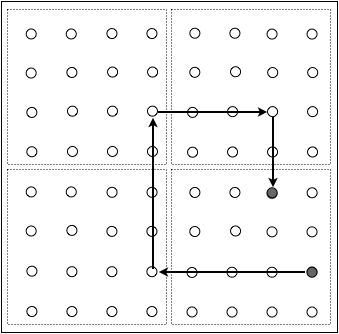
\includegraphics[scale=0.4]{FiguresGraph/routingCitySolution1}
       \caption{To discuss.}
  \label{fig:routingCity}
\end{center}
\end{figure}
 \begin{figure}[hbt]
\begin{center}
       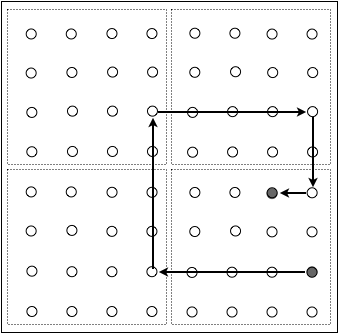
\includegraphics[scale=0.4]{FiguresGraph/routingCity2}
       \caption{To discuss.}
%  \label{fig:routingCity}
\end{center}
\end{figure}
 \begin{figure}[hbt]
\begin{center}
       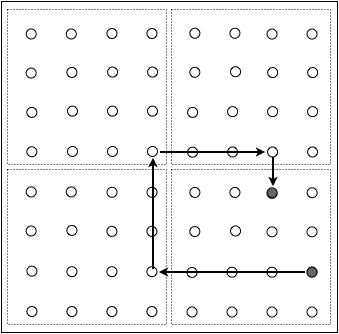
\includegraphics[scale=0.4]{FiguresGraph/routingCity3}
       \caption{Shortest path.}
%  \label{fig:routingCity}
\end{center}
\end{figure}

\end{itemize}


%%%%%%%%%%%%%%%%%%%%%%%%%%%%%%%%%%%%%%%%
%\section*{Exercises Chapter 13}

\begin{itemize}
\item
{\bf 13.2. Appreciating de Bruijn networks}
\smallskip


\noindent
{\em a. Identify, by coloring the edges of $\d_3$ and $\d_4$, how each network can be viewed as two trees which are ``embracing" one another.}

\smallskip

Fig.~\ref{fig:DeBruijn3Tree} shows both trees for $\d_3$. 
The first one is rooted at the extreme left while the second one is rooted at the extreme right of the figure. 
\begin{figure}[h]
\begin{center}
        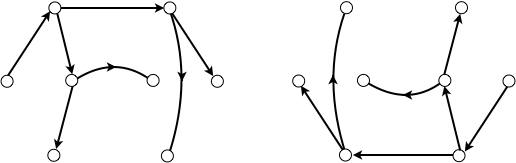
\includegraphics[scale=0.4]{FiguresGraph/DeBruijn3Tree}
        \caption{Two interleaved trees in $\d_3$.}
        \label{fig:DeBruijn3Tree}
\end{center}
\end{figure}


\medskip\item 
{\bf 13.4. Fundamental insights into outerplanarity in graphs}
\smallskip

{\em Prove the following assertions.}

\noindent {\em a. Show that the complete bipartite graph $K_{3,2}$ is not outerplanar.}
\smallskip

The question is how to distribute the two groups of vertices (dark grey and white) on a circle
with no crossing edges.
The solution is a case by case analysis according to all the possibilities to distribute $K_{3,2}$'s vertices around a circle:
either the vertices of each of both groups are distributed consecutively, or each group of vertices is interlaced with a vertex of the other group.
Fig.~\ref{fig:outerplanarK32} depictes both cases.

Int is easy to verify that in each case, it is impossible to link the isolated white vertex with the three dark grey ones.

\begin{figure}[h]
\begin{center}
        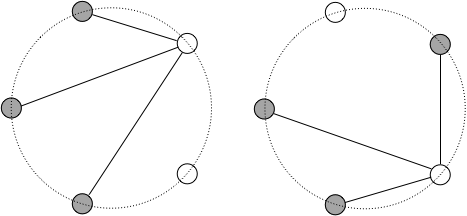
\includegraphics[scale=0.4]{FiguresGraph/outerplanarK3,2}
        \caption{The two only possibilities to distribute the white and shaded vertices along a circle.}
        \label{fig:outerplanarK32}
\end{center}
\end{figure}


\end{itemize}


